\section{Systemmodelle}
% TODO T Nummern anpassen

\subsection{Objektmodelle}
% UML Klassendiagramme

\begin{figure}[H]
\centering
\includegraphics[scale=0.5]{../system_models/object_models/lambda_calculus.pdf}
\caption{UML Klassendiagramm zum Lambda-Kalkül}
\end{figure}

\subsection{Dynamische Modelle}
% UML Zustandsautomat, Sequenzdiagramm

%\newgeometry{left=40pt}
\begin{figure}[H]
\centering
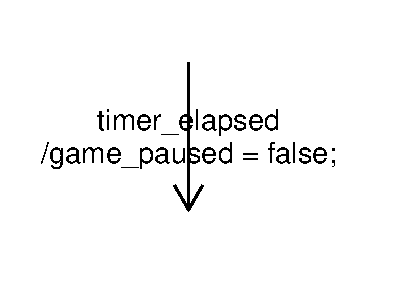
\includegraphics[scale=0.4]{../system_models/dynamic_models/menu_state_machine.pdf}
\caption{Zustandsautomat zur Menübedienung}
\end{figure}
%\restoregeometry

\begin{figure}[H]
\centering
\includegraphics[scale=0.55]{../system_models/dynamic_models/game_level_state_machine.pdf}
\caption{Zustandsautomat zum Ablauf eines Levels}
\end{figure}

\begin{figure}[H]
\centering
\includegraphics[scale=0.55]{../system_models/dynamic_models/reduction_mode_state_machine.pdf}
\caption{Zustandsautomat zur Funktion des Reduktions-Modus}
\end{figure}

\subsection{Benutzerschnittstelle}

GUI